% kapitel5.tex
\chapter{Optimization Studies for the Event Selection}

\section{Search for Discriminating Variables }
The first part of the optimization studies is the search for variables which provide a significant distinction between background and signal.
Caused by the basic selection discussed in section \ref{basic selection} there is already much background rejected.
Moreover the requirement of two large-R jets cause that the remaining background events contain high energies, because large-R jets, which fulfill the minimum criteria, have to be produced.
This complicates the search for discriminating variables, because the signal is expected to contain high energies,too, because of the massive vector-like quarks.\\
Figure \ref{H_T} shows the distribution for the scalar sum of the transverse momenta of all jets in an event.

\begin{figure}
\centering
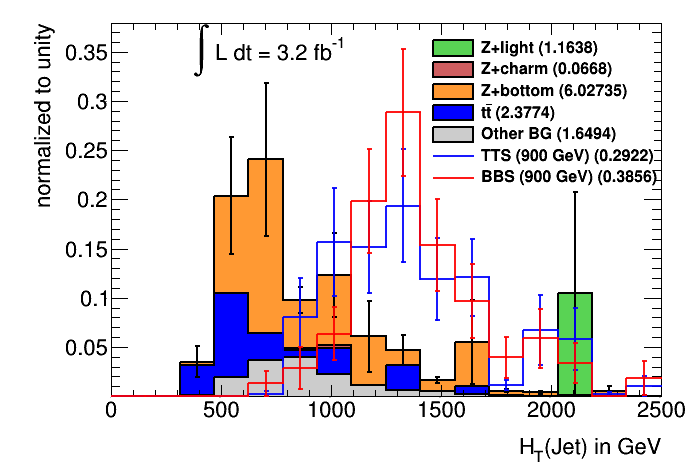
\includegraphics[width=8cm]{figures/H_T.png}
\caption{Plot for the scalar sum of all jet $p_{T}$'s in an event after the preselection. 
Both signal and background are presented and the distributions are normalized to unity. 
The weighted number of events is displayed in the legend in brackets next to the processes. 
The number of events are expected for a integrated luminosity $\int L dt$ = \SI{3.2}{fb^{-1}}}
\label{H_T}
\end{figure}

The distribution shows, that the signal is shifted to the right compared to the background, because there is more energy in the events resulting from the very massive vector-like quarks. 
Figure \ref{Zpt} presents the distribution of the Z candidate $p_{T}$.
\begin{figure}
\centering
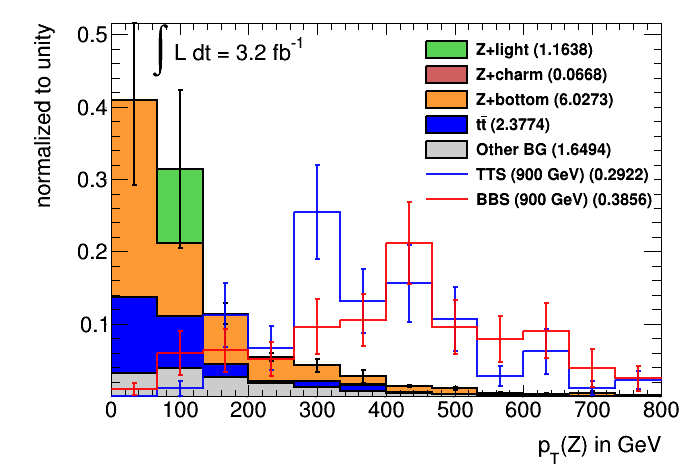
\includegraphics[width=8cm]{figures/Zpt.png}
\caption{Plot for the Z candidate $p_{T}$. 
Both signal and background are presented and the distributions are normalized to unity. 
The weighted number of events is displayed in the legend in brackets next to the processes. 
The number of events are expected for a integrated luminosity $\int L dt$ = \SI{3.2}{fb^{-1}}}
\label{Zpt}
\end{figure}

As mentioned for the $H_{T}$-distribution the signal is shifted to the right. That is as expeced, because the Z candidate results straight from the vector-like quark and should have a $p_{T}$ about \SI{450}{GeV}.
In figure \ref{leadingljet} the $p_{T}$ of the leading large-R jet is represented, which means the $p_{T}$ of the large-R jets with the highest $p_{T}$ in an event.
\vspace{-0.5cm}
\begin{figure}[h!]
\centering
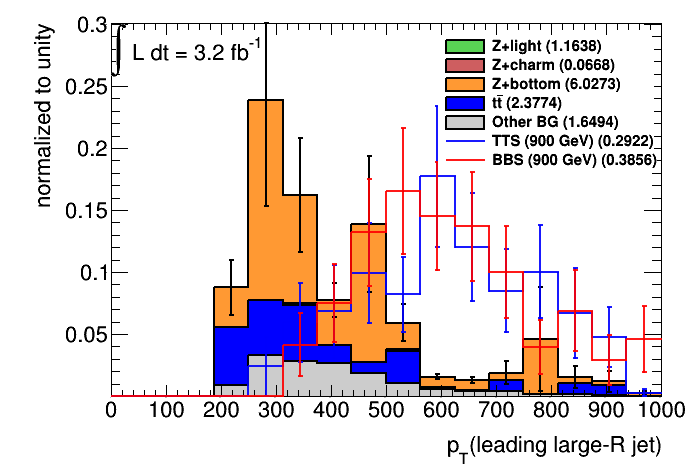
\includegraphics[width=8cm]{figures/leadingljet.png}
\caption{Plot for the leading large-R jet $p_{T}$. 
Both signal and background are presented and the distributions are normalized to unity. 
The weighted number of events is displayed in the legend in brackets next to the processes. 
The number of events are expected for a integrated luminosity $\int L dt$ = \SI{3.2}{fb^{-1}}.}
\label{leadingljet}
\end{figure}

Figure \ref{mZb} shows the distribution of the invariant mass of the Z candidate and the highest $p_{T}$ b-jet and \ref{mZt} the invariant mass of the Z candidate and the highest $p_{T}$ top-jet.


%\resizebox{0.48\columnwidth}{!}{
\begin{figure}[h]
    \centering
    \resizebox{0.46\columnwidth}{!}{
    \begin{subfigure}{.49\textwidth}
      \centering
      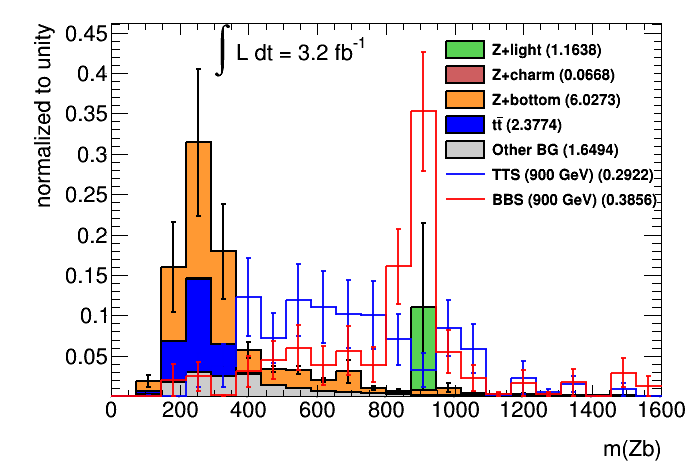
\includegraphics[width=.99\linewidth]{figures/mZb.png}
      \caption{}
      \label{mZb}
    \end{subfigure}
    }
    \resizebox{0.46\columnwidth}{!}{
    \begin{subfigure}{.49\textwidth}
      \centering
      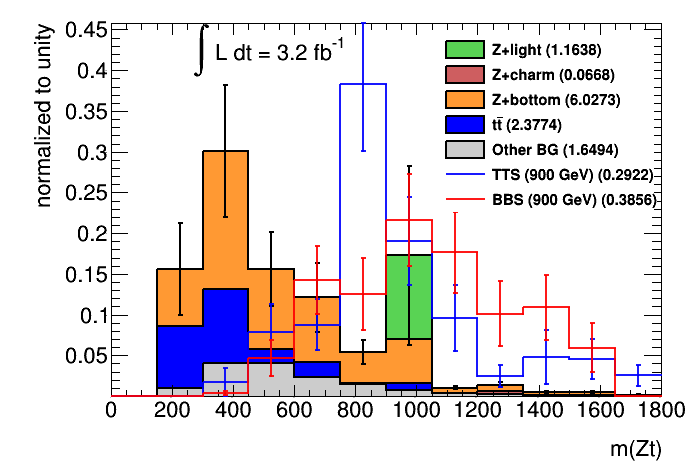
\includegraphics[width=.99\linewidth]{figures/mZt.png}
      \caption{}
      \label{mZt}
    \end{subfigure}
    }
    \caption{Plot for the invariant mass of the Z candidate and the highest $p_{T}$ b-jet (a) and the invariant mass of the Z candidate and the highest $p_{T}$ top-jet (b)  . 
Both signal and background are presented and the distributions are normalized to unity. 
The weighted number of events is displayed in the legend in brackets next to the processes. 
The number of events are expected for a integrated luminosity $\int L dt$ = \SI{3.2}{fb^{-1}}.}
    \label{fig::stop}   
\end{figure}
%}
The signal is shifted to the right caused by the same argumentation mentioned before. 
For the BBS signal process there is a peak at \SI{900}{GeV} in figure \ref{mZb}.
This is as expected because the Z candidate and the highest $p_{T}$ b-jet should result from the vector-like quark decay B \texorpdfstring{$\longrightarrow$}~Zb.
For the peak 


\section{Significance for Different Cuts}

\section{Proposel for a Boosted Event Selection}

